\documentclass[12pt, a4paper]{article}

% --- Pakiety ---
\usepackage[utf8]{inputenc}
\usepackage[T1]{fontenc}
\usepackage[polish]{babel}
\usepackage{geometry}
\usepackage{amsmath}
\usepackage{amssymb}
\usepackage{graphicx}
\usepackage{booktabs}
\usepackage{siunitx}
\usepackage{caption}
\usepackage{subcaption}
\usepackage{float}
\usepackage{hyperref}
\usepackage{xcolor}
\usepackage{array}
\usepackage{multirow}
\usepackage{fancyhdr}

% --- Marginesy ---
\geometry{
    top=2.5cm,
    bottom=2.5cm,
    left=2.5cm,
    right=2.5cm
}

% --- Stopka ---
\pagestyle{fancy}
\fancyhf{}
\renewcommand{\headrulewidth}{0pt}
\renewcommand{\footrulewidth}{0.4pt}
\fancyfoot[R]{
\includegraphics[height=0.8cm]{lumon.pdf}}

% --- Konfiguracja siunitx ---
\sisetup{
    output-decimal-marker = {,},
    separate-uncertainty = true
}

% --- Dane raportu ---
\newcommand{\tytul}{Wyznaczanie ciepła topnienia lodu}
\newcommand{\codeword}{Trinity}
\newcommand{\nrCwiczenia}{C4}
\newcommand{\autor}{Karol Peszek}
\newcommand{\nrGrupy}{Grupa B}
\newcommand{\dataWykonania}{25 marca 2026}

% --- Tytuł dokumentu ---
\title{
    \large I Pracownia Fizyczna \\[0.5em]
    \textbf{Ćwiczenie \nrCwiczenia} \\[0.3em]
    \LARGE \tytul\space''\codeword''
}
\author{
    \autor\\
     Grupa \nrGrupy}
\date{
    Data wykonania pomiarów: \dataWykonania\\
}

% =============================================
\begin{document}
% =============================================

\maketitle
\thispagestyle{empty}
\newpage

% -------------------------------------------
\section{Cel ćwiczenia}
% -------------------------------------------
Celem ćwiczenia jest wyznaczenie ciepła topnienia lodu poprzez pomiar
temperatury i masy wody oraz lodu zakładając, że kalorymetr jest idealnie
izolowany termicznie. W dalszej części ćwiczenia zostanie również wyznaczone
ciepło właściwe kalorymetru zbudowanego z aluminium.

% -------------------------------------------
\section{Wstęp teoretyczny}
% -------------------------------------------

\subsection{Energia wewnętrzna, ciepło i temperatura}
Każda substancja zbudowana jest z ogromnej liczby cząsteczek, które nigdy nie
pozostają w całkowitym spoczynku --- wykonują nieustanny, chaotyczny ruch. Całość
energii związanej z tym ruchem oraz wzajemnymi oddziaływaniami między
cząsteczkami określa się mianem energii wewnętrznej układu. Temperatura jest
miarą przeciętnej energii kinetycznej cząsteczek --- im intensywniejszy ich ruch,
tym wyższa temperatura. Bezwzględne zero (\qty{0}{\kelvin}) odpowiada
teoretycznemu stanowi całkowitego zatrzymania ruchu cząsteczek.

Gdy dwa ciała o różnych temperaturach się stykają, cząsteczki na
ich powierzchni granicznej zaczną wymieniać energię kinetyczną. W rezultacie
cieplejsze ciało oddaje energię chłodniejszemu. Energię
przekazywaną drogą kontaktu termicznego nazywamy ciepłem. Ilość ciepła
potrzebna do podgrzania jednostki masy danej substancji o jeden kelwin jest stałą dla danego materiału
zwaną ciepłem właściwym $c$. Związek między dostarczoną
energią $Q$, masą ciała $m$ a zmianą temperatury $\Delta T$ opisuje zależność:
\begin{equation}
    Q = cm\Delta T.
\end{equation}

Zasada zachowania energii w termodynamice --- pierwsza zasada termodynamiki ---
mówi, że zmiana energii wewnętrznej układu jest sumą ciepła przekazanego do
układu i pracy wykonanej nad układem. W praktyce wyznaczania ciepła przemiany
fazowej oznacza to, że w układzie odizolowanym ciepło oddane przez jedne
składniki musi zostać pochłonięte przez pozostałe. Ten bilans cieplny stanowi
podstawę działania kalorymetru --- naczynia zminimalizowanego termicznie od
otoczenia (najczęściej obudowanego izolatorem, z posrebrzanymi ściankami
ograniczającymi straty na promieniowanie).

Materia na Ziemi występuje w trzech stanach skupienia: stałym, ciekłym i
gazowym. W ciele stałym cząsteczki są trwale związane w określonych
położeniach, w cieczy oddziaływania są słabsze, a w gazie praktycznie zanikają.
Przejście między stanami skupienia wymaga dostarczenia --- lub powoduje
wydzielenie --- określonej ilości energii, mimo że temperatura substancji w
trakcie przemiany pozostaje stała. Dzieje się tak, ponieważ dostarczana energia
nie zwiększa energii kinetycznej cząsteczek, lecz jest w całości zużywana na
zerwanie wiązań między nimi, czyli na wzrost energii potencjalnej. Tę energię,
związaną z przemianą fazową, a nie ze zmianą temperatury, nazywamy ciepłem
utajonym lub ciepłem przemiany.

\subsection{Ciepło topnienia lodu}
W przypadku topnienia lodu ciepło topnienia $q_t$ to ilość energii potrzebna do
stopienia jednostki masy substancji w temperaturze topnienia. Jeśli do
kalorymetru z wodą o masie $m_w$ i temperaturze $T_p$ wrzucimy osuszone kawałki
lodu o masie $m_l$ (w temperaturze \qty{0}{\degreeCelsius}), to po jego
całkowitym roztopieniu ustali się temperatura końcowa $T_k$. Energia oddana
przez wodę i kalorymetr (o masie $m_k$ i cieple właściwym $c_k$) zostaje zużyta
na stopienie lodu oraz podgrzanie powstałej wody do $T_k$. Z bilansu cieplnego:
\begin{equation}
    (m_w c_w + m_k c_k)(T_p - T_k) = m_l\left[q_t + c_w T_k\right],
\end{equation}
skąd wyznacza się ciepło topnienia lodu:
\begin{equation}
    q_t = \frac{(c_w m_w + c_k m_k)(T_p - T_k)}{m_l} - c_w T_k.
    \label{eq:qt}
\end{equation}

Ważnym warunkiem eksperymentu jest użycie starannie osuszonego lodu --- nawet
niewielka ilość wody na jego powierzchni wprowadza istotny błąd systematyczny
do bilansu cieplnego.

\subsection{Ciepło właściwe kalorymetru}

Do wyznaczenia ciepła właściwego kalorymetru $c_k$ wykorzystuje się mieszanie
dwóch porcji wody w różnych temperaturach. Do kalorymetru wlewa się zimną wodę
o masie $m_z$ i temperaturze $T_z$, a następnie po ustaleniu się temperatury
dolewa się gorącą wodę o masie $m_g$ i temperaturze $T_g$. Po wymieszaniu i
ustaleniu się temperatury końcowej $T_k$ bilans cieplny ma postać:

\begin{equation}
    m_g c_w (T_g - T_k) = (m_z c_w + m_k c_k)(T_k - T_z),
\end{equation}
gdzie $c_w$ jest ciepłem właściwym wody. Stąd ciepło właściwe kalorymetru:
\begin{equation}
    c_k = \frac{m_g c_w (T_g - T_k) - m_z c_w (T_k - T_z)}{m_k (T_k - T_z)}.
    \label{eq:ck}
\end{equation}

Masę dolanej gorącej wody $m_g$ wyznacza się przez zważenie kalorymetru przed i
po dolaniu wody.

% -------------------------------------------
\subsection{Przyjęte wartości stałe}
% -------------------------------------------
\subsubsection{Pomiar ciepła topnienia lodu}
Do wyznaczenia ciepła topnienia lodu z bilansu cieplnego~\eqref{eq:qt} należy
znać ciepło wartość ciepła właściwego wody oraz kalorymetru (zbudowanego z
aluminium). W ćwiczeniu przyjęto następujące wartości:

\begin{itemize}
    \item Ciepło właściwe wody: $c_w = \qty{4187}{\joule\per\kilogram\per\kelvin}$~\cite{skrypt},
    \item Ciepło właściwe aluminium: $c_{Al} = \qty{897}{\joule\per\kilogram\per\kelvin}$~\cite{emetal}.
\end{itemize}

\subsubsection{Pomiar ciepła właściwego kalorymetru}
Do wyznaczenia ciepła właściwego kalorymetru z bilansu cieplnego~\eqref{eq:ck}
również potrzebne jest ciepło właściwe wody, które przyjęto jako $c_w =
    \qty{4187}{\joule\per\kilogram\per\kelvin}$~\cite{skrypt}.

% -------------------------------------------
\section{Opis układu pomiarowego}
% -------------------------------------------
\begin{figure}[H]
    \centering
    
\includegraphics[width=1\textwidth]{schema.jpg}
    \caption{Schemat układu pomiarowego.}\label{fig:schemat}
\end{figure}

\subsection{Przyrządy użyte do przeprowadzenia eksperymentu}
W ćwiczeniu wykorzystano następujące przyrządy pomiarowe:
\begin{itemize}
    \item kalorymetr:
    \begin{itemize}
        \item wewnętrzna częśc kalorymetru wykonana z aluminium,
        \item zewnętrzna część kalorymetru wykonana z aluminium,
        \item pokrywka wykonana z z otworami na termometr i mieszadełko,
        \item mieszadełko wykonane z aluminium,
        \item termometr o podziałce \qty{0.2}{\degreeCelsius} i zakresie pomiarowym od \qty{10}{\degreeCelsius} do \qty{50}{\degreeCelsius},
    \end{itemize}
    \item waga elektryczna AXIS B2 o zakresie pomiarowym do \qty{2000}{\gram} i dokładności \qty{0.1}{\gram},
    \item plastikowa zlewka,
    \item ręczniki papierowe,
    \item odstana woda w temperaturze pokojowej,
    \item ciepła i zimna woda z kranu,
    \item kostki lodu z zamrażarki w temperaturze \qty{0}{\degreeCelsius} osuszone ręcznikiem papierowym.
\end{itemize}

\subsection{Opis układu pomiarowego}
Kalorymetr składa się z części wewnętrznej i zewnętrznej wykonanych z aluminium. Między naczyniami znajduje się powietrze które pełni rolę izolatora termicznego. Otwory w plastikowej poklrywce umożliwiają wprowadzenie termometru i mieszadełka, które służą do pomiaru temperatury i mieszania zawartości kalorymetru. Waga elektryczna służy do precyzyjnego ważenia masy kalorymetru oraz masy wody i lodu. Zlewka jest używana do przygotowania odpowiednich ilości wody, a ręczniki papierowe służą do osuszania kostek lodu przed ich umieszczeniem w kalorymetrze, co jest kluczowe dla uniknięcia błędów systematycznych w bilansie cieplnym.
% -------------------------------------------
\section{Procedura pomiarowa}
% -------------------------------------------
Pomiary przeprowadzono w dniu 25.03.2026 roku. Procedura pomiarowa składała się z następujących kroków:

\subsection{Pomiar ciepła topnienia lodu}
Wykonano 4 serier pomiarowe. W każdej serii wykonano następujące czynności:
\begin{enumerate}
    \item Przygotowanie układu pomiarowego zgodnie z rysunkiem~\ref{fig:schemat}.
    \item Nalanie wewnętrznej części kalorymetru wody.
    \item Zważenie kalorymetru z wodą i mieszadełkiem.
    \item Włożenie wewnętrznej części z wodą do zewnętrznej części kalorymetru.
    \item Odczekanie do ustalenia się temperatury w kalorymetrze i zapisanie odczytu termometru jako temperatury początkowej $T_p$.
    \item Osuszenie ręcznikiem papierowym kostek lodu i wrzucenie ich do kalorymetru.
    \item Mieszanie zawartości kalorymetru do momentu całkowitego roztopienia lodu i ustalenia się temperatury końcowej $T_k$ i zapisanie jej.
    \item Wyjęcie środkowej części kalorymetru z wodą i roztopionym lodem i zważenie jej w celu wyznaczenia masy lodu $m_l$.
    \item Opróżnienie kalorymetru, osuszenie go i przygotowanie do kolejnej serii pomiarowej.
\end{enumerate}

\subsection{Pomiar ciepła właściwego kalorymetru}
Wykonano jedną serię pomiarową. W serii wykonano następujące czynności:
\begin{enumerate}
    \item Przygotowanie układu pomiarowego zgodnie ze zdjęciem schematu~\ref{fig:schemat}.
    \item Nalanie zimnej wody do wewnętrznej części kalorymetru.
    \item Zważenie kalorymetru z zimną wodą i mieszadełkiem.
    \item Włożenie wewnętrznej części z zimną wodą do zewnętrznej części kalorymetru.
    \item Odczekanie do ustalenia się temperatury w kalorymetrze i zapisanie odczytu termometru jako temperatury zimnej wody $T_z$.
    \item Zważeniem pustej zlewki i zważenie jej po nalaniu gorącej wody w celu wyznaczenia masy gorącej wody $m_g$.
    \item Ustalenie temperatury gorącej wody $T_g$ poprzez zanurzenie termometru w zlewce z gorącą wodą i zapisanie odczytu.
    \item Wylanie gorącej wody do kalorymetru z zimną wodą.
    \item Mieszanie zawartości kalorymetru do momentu ustalenia się temperatury końcowej $T_k$ i zapisanie jej.
    \item Opróżnienie kalorymetru i osuszenie go.
\end{enumerate}




% -------------------------------------------
\section{Wyniki pomiarów}
% -------------------------------------------
Szczegółowe wyniki pomiarów znajdują się w zeszycie pomiarowym oraz w dostarczonych
plikach csv.
Masy mierzono pięciokrotnie wagą elektryczną ($u_m = \qty{0{,}1}{\gram}$); temperatury mierzono jednokrotnie
termometrem o podziałce $\qty{0{,}2}{\degreeCelsius}$ ($u_T = \qty{0{,}2}{\degreeCelsius}$).
W~wierszu \textit{śr.} podano średnią arytmetyczną, a~w~wierszu $u$ --- złożoną niepewność standardową
$u = \sqrt{u_A^2 + u_B^2}$, gdzie $u_A = s/\!\sqrt{N}$.

\subsection{Masa pustej części wewnętrznej kalorymetru}\label{sec:wyniki_mk}

Masa wewnętrznej części kalorymetru wraz z mieszadełkiem~$m_k$ jest wielkością wspólną dla obu
eksperymentów i~wyznaczono ją jednokrotnie.

\begin{table}[H]
\centering
\caption{Pięciokrotny pomiar masy wewnętrznej części kalorymetru z mieszadełkiem~$m_k$.}\label{tab:mk}
\begin{tabular}{c S[table-format=3.2]}
\toprule
Lp. & {$m_k$ [\unit{\gram}]} \\
\midrule
1 & 133.6 \\
2 & 133.7 \\
3 & 133.5 \\
4 & 133.7 \\
5 & 133.7 \\
\midrule
{śr.} & 133.64 \\
{$u$}  & {$\qty{0{,}11}{\gram}$} \\
\bottomrule
\end{tabular}
\end{table}

\subsection{Wyznaczanie ciepła właściwego kalorymetru}\label{sec:wyniki_qal}
Wyniki bezpośrednich pomiarów dla wyznaczania ciepła właściwego kalorymetru zostały przedstawione poniżej:
\begin{table}[H]
\centering
\caption{Wielokrotne pomiary mas podczas wyznaczania ciepła właściwego kalorymetru.
         $m_{\mathrm{zl},0}$ --- masa pustej zlewki;
         $m_{\mathrm{zl}}$ --- masa zlewki z gorącą wodą;
         $m_{k,z}$ --- masa kalorymetru z mieszadełkiem i zimną wodą.}\label{tab:qal_masy}
\begin{tabular}{c
    S[table-format=2.2]
    S[table-format=3.2]
    S[table-format=3.2]}
\toprule
Lp. & {$m_{\mathrm{zl},0}$ [\unit{\gram}]} & {$m_{\mathrm{zl}}$ [\unit{\gram}]} & {$m_{k,z}$ [\unit{\gram}]} \\
\midrule
1 & 56.8 & 248.0 & 418.7 \\
2 & 56.7 & 247.9 & 418.6 \\
3 & 56.7 & 247.9 & 418.6 \\
4 & 56.6 & 247.9 & 418.6 \\
5 & 56.7 & 247.9 & 418.5 \\
\midrule
{śr.} & 56.70 & 247.92 & 418.60 \\
{$u$}  & {$\qty{0{,}10}{\gram}$} & {$\qty{0{,}10}{\gram}$} & {$\qty{0{,}10}{\gram}$} \\
\bottomrule
\end{tabular}
\end{table}

\begin{table}[H]
\centering
\caption{Jednokrotne pomiary temperatur podczas wyznaczania ciepła właściwego kalorymetru.}\label{tab:qal_temp}
\begin{tabular}{l S[table-format=2.1]}
\toprule
Wielkość & {Wartość [\unit{\degreeCelsius}]} \\
\midrule
Temperatura gorącej wody w zlewce $T_g$                   & 35.8 \\
Temperatura wody w kalorymetrze przed dolaniem $T_z$       & 10.2 \\
Temperatura wody w kalorymetrze po dolaniu $T_k$           & 20.0 \\
\bottomrule
\end{tabular}
\end{table}

\begin{table}[H]
\centering
\caption{Masy pochodne wyznaczone podczas pomiaru ciepła właściwego kalorymetru.
         $m_g = \bar{m}_{\mathrm{zl}} - \bar{m}_{\mathrm{zl},0}$ --- masa gorącej wody;
         $m_z = \bar{m}_{k,z} - \bar{m}_k$ --- masa zimnej wody.
         Niepewności: $u = \sqrt{u_A^2 + u_B^2}$.}\label{tab:qal_mg_mz}
\begin{tabular}{l S[table-format=3.2] S[table-format=1.2]}
\toprule
Wielkość & {Wartość [\unit{\gram}]} & {$u$ [\unit{\gram}]} \\
\midrule
$m_g$ (gorąca woda)  & 191.22 & 0.14 \\
$m_z$ (zimna woda)   & 284.96 & 0.15 \\
\bottomrule
\end{tabular}
\end{table}

\subsection{Wyznaczanie ciepła topnienia lodu}\label{sec:wyniki_qt}

Pomiary przeprowadzono w czterech seriach. W każdej serii masę kalorymetru z wodą ważono
pięciokrotnie (przed dodaniem i po roztopieniu lodu); temperatury mierzono jednokrotnie.
Niepewności jak w sekcji~\ref{sec:wyniki_qal}.

\begin{table}[H]
\centering
\caption{Wielokrotne pomiary masy kalorymetru z wodą i mieszadełkiem \textbf{przed} dodaniem lodu
         $m_{\mathrm{przed}}$ [\unit{\gram}].}\label{tab:qt_przed}
\begin{tabular}{c
    S[table-format=3.1]
    S[table-format=3.1]
    S[table-format=3.1]
    S[table-format=3.1]}
\toprule
Lp. & {Seria 1} & {Seria 2} & {Seria 3} & {Seria 4} \\
\midrule
1 & 663.3 & 490.8 & 538.9 & 652.1 \\
2 & 663.2 & 490.9 & 538.8 & 652.0 \\
3 & 663.3 & 490.9 & 538.8 & 652.1 \\
4 & 663.2 & 490.9 & 538.9 & 652.0 \\
5 & 663.2 & 490.9 & 538.8 & 652.1 \\
\midrule
{śr.} & 663.24 & 490.88 & 538.84 & 652.06 \\
{$u$} & {$\qty{0{,}10}{\gram}$} & {$\qty{0{,}10}{\gram}$}
      & {$\qty{0{,}10}{\gram}$}  & {$\qty{0{,}10}{\gram}$} \\
\bottomrule
\end{tabular}
\end{table}

\begin{table}[H]
\centering
\caption{Wielokrotne pomiary masy kalorymetru z wodą i mieszadełkiem \textbf{po} roztopieniu lodu
         $m_{\mathrm{po}}$ [\unit{\gram}].}\label{tab:qt_po}
\begin{tabular}{c
    S[table-format=3.1]
    S[table-format=3.1]
    S[table-format=3.1]
    S[table-format=3.1]}
\toprule
Lp. & {Seria 1} & {Seria 2} & {Seria 3} & {Seria 4} \\
\midrule
1 & 716.3 & 599.5 & 652.0 & 653.0 \\
2 & 716.2 & 599.5 & 651.8 & 652.9 \\
3 & 716.3 & 599.5 & 651.8 & 652.9 \\
4 & 716.3 & 599.4 & 651.9 & 652.9 \\
5 & 716.2 & 599.5 & 651.8 & 652.9 \\
\midrule
{śr.} & 716.26 & 599.48 & 651.86 & 652.92 \\
{$u$} & {$\qty{0{,}10}{\gram}$}  & {$\qty{0{,}10}{\gram}$}
      & {$\qty{0{,}11}{\gram}$}  & {$\qty{0{,}10}{\gram}$} \\
\bottomrule
\end{tabular}
\end{table}

\begin{table}[H]
\centering
\caption{Masa wody w kalorymetrze przed dodaniem lodu per seria,
         $m_w = \bar{m}_{\mathrm{przed}} - \bar{m}_k$,
         z niepewnością $u_{m_w} = \sqrt{u_{\bar{m}_{\mathrm{przed}}}^2 + u_{\bar{m}_k}^2}$.}\label{tab:qt_mw}
\begin{tabular}{c S[table-format=3.2] S[table-format=1.3]}
\toprule
Seria & {$m_w$ [\unit{\gram}]} & {$u_{m_w}$ [\unit{\gram}]} \\
\midrule
1 & 529.60 & 0.15 \\
2 & 357.24 & 0.15 \\
3 & 405.20 & 0.15 \\
4 & 518.42 & 0.15 \\
\bottomrule
\end{tabular}
\end{table}

\begin{table}[H]
\centering
\caption{Masa lodu dosypanego w każdej serii,
         $m_l = \bar{m}_{\mathrm{po}} - \bar{m}_{\mathrm{przed}}$,
         z niepewnością $u_{m_l} = \sqrt{u_{\bar{m}_{\mathrm{po}}}^2 + u_{\bar{m}_{\mathrm{przed}}}^2}$.}\label{tab:qt_ml}
\begin{tabular}{c S[table-format=3.2] S[table-format=1.3]}
\toprule
Seria & {$m_l$ [\unit{\gram}]} & {$u_{m_l}$ [\unit{\gram}]} \\
\midrule
1 &  53.02 & 0.146 \\
2 & 108.60 & 0.144 \\
3 & 113.02 & 0.149 \\
4 &   0.86 & 0.145 \\
\bottomrule
\end{tabular}
\end{table}

\begin{table}[H]
\centering
\caption{Jednokrotne pomiary temperatur wody w kalorymetrze przed dodaniem i po roztopieniu lodu.}\label{tab:qt_temp}
\begin{tabular}{c S[table-format=2.1] S[table-format=2.1]}
\toprule
Seria & {$T_p$ [\unit{\degreeCelsius}]} & {$T_k$ [\unit{\degreeCelsius}]} \\
\midrule
1 & 21.0 & 12.6 \\
2 & 36.4 & 11.2 \\
3 & 40.6 & 16.2 \\
4 & 40.6 & 19.0 \\
\bottomrule
\end{tabular}
\end{table}

% -------------------------------------------
\section{Opracowanie wyników}
% -------------------------------------------

\subsection{Ciepło właściwe kalorymetru}

Na podstawie wyników z tabel~\ref{tab:qal_masy},~\ref{tab:qal_temp} i~\ref{tab:qal_mg_mz}
oraz wzoru~\eqref{eq:ck} obliczono ciepło
właściwe kalorymetru. Propagację niepewności przeprowadzono metodą kwadratury
(pierwiastek z~sumy kwadratów składowych). Wynik:
\begin{equation}
    c_k = \qty{731 \pm 395}{\joule\per\kilogram\per\kelvin}.
\end{equation}
Dominującym źródłem niepewności (65{,}4\,\% wariancji) jest pomiar temperatury~$T_k$,
co wynika z~małej różnicy temperatur $(T_k - T_z) = \qty{9{,}8}{\kelvin}$ w~mianowniku
wzoru --- pochodna $\partial c_k/\partial T_k \propto {(T_k-T_z)}^{-2}$ jest tym większa,
im bliższe są temperatury zimnej i~gorącej porcji wody.
Dla porównania tablicowa wartość ciepła właściwego aluminium wynosi
$c_{\mathrm{Al}} = \qty{897}{\joule\per\kilogram\per\kelvin}$.

\subsection{Ciepło topnienia lodu}

\subsubsection{Odrzucenie serii 4}

W~serii~4 zmierzona masa lodu wynosi $m_l = \qty{0{,}86}{\gram}$, co odpowiada
śladowej ilości lodu w~kalorymetrze --- analogiczna wartość w~seriach 1--3 wynosi
od \qty{53}{\gram} do \qty{113}{\gram}. Prawdopodobną przyczyną jest błędne zapisanie wyników w zeszycie pomiarowym, gdyż strony z pomiarami były kopiowane między seriami aby zaoszczędzić czas na pisaniu wspólnych części. Seria~4 została więc wykluczona z~dalszej analizy.

\subsubsection{Ciepło właściwe kalorymetru}
Ciepło właściwe kalorymetru wyznaczone w poprzedniej sekcji jest zgodne w granicy niepewności z wartością tablicową, jednak jest obarczone dużym błędem rzędu 54{,}0\,\%. Z tego powodu zdecydowano się na użycie wartości tablicowej $c_k = \qty{897}{\joule\per\kilogram\per\kelvin}$ do dalszych obliczeń ciepła topnienia lodu.

\subsubsection{Wyniki serii 1--3}

Wyniki obliczone ze wzoru~\eqref{eq:qt} dla serii 1--3 zestawiono
w~tabeli~\ref{tab:qt_wyniki}.

\begin{table}[H]
\centering
\caption{Wyznaczone ciepło topnienia lodu $q_t$ dla serii 1--3.}\label{tab:qt_wyniki}
\begin{tabular}{c S[table-format=6.0] S[table-format=5.0]}
\toprule
Seria & {$q_t$ [\unit{\joule\per\kilogram}]} & {$u_{q_t}$ [\unit{\joule\per\kilogram}]} \\
\midrule
1 & 317609 & 13120 \\
2 & 328098 &  4872 \\
3 & 324412 &  5207 \\
\bottomrule
\end{tabular}
\end{table}

\subsubsection{Wynik końcowy}

Ostateczna wartość ciepła topnienia lodu wyznaczona jako ważona średnia
z~serii 1--3 (wagi $w_i = 1/u_i^2$):
\refstepcounter{equation}\label{eq:qt_wynik}\(q_t = \qty{325784 \pm 3433}{\joule\per\kilogram} \approx \qty[separate-uncertainty=true]{326(3)}{\kilo\joule\per\kilogram}.\)
Wyniki pomiarowe wraz ze średnią ważoną i~wartością tablicową przedstawiono
na rysunku~\ref{fig:qt_wyniki}.

\begin{figure}[H]
\centering
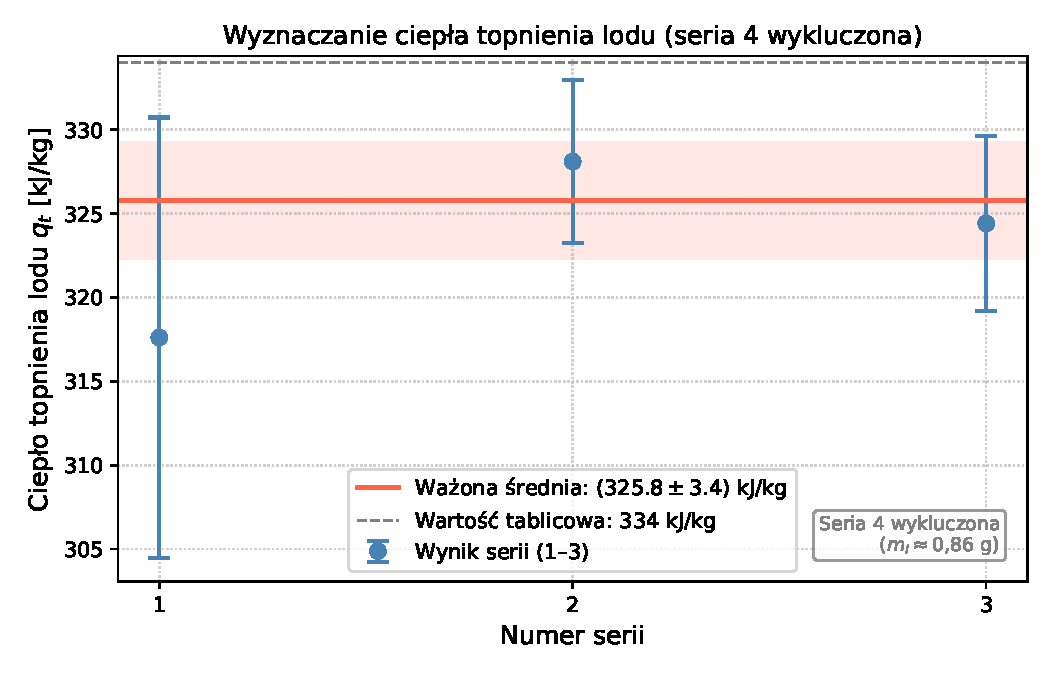
\includegraphics[width=0.82\textwidth]{qt_results.pdf}
\caption{Wyznaczone ciepło topnienia lodu dla serii 1--3 z~niepewnościami pomiarowymi.
         Linia czerwona --- ważona średnia~\eqref{eq:qt_wynik};
         pasmo --- jej niepewność;
         linia szara przerywana --- wartość tablicowa \qty{334}{\kilo\joule\per\kilogram}.
         Seria~4 ($m_l \approx \qty{0{,}86}{\gram}$) została wykluczona.}\label{fig:qt_wyniki}
\end{figure}

% -------------------------------------------
\section{Wnioski}
% -------------------------------------------
\subsection{Ciepło właściwe kalorymetru}
Wyznaczone ciepło właściwe kalorymetru jest zgodne z~wartością tablicową, jednak obarczone dużym błędem. Jako przyczyny można wymienić między innymi wylanie się drobnej ilości wody podczas wlewania gorącej wody do kalorymetru, co skutkowało niedokładnym określeniem masy zimnej wody $m_z$ i~masy gorącej wody $m_g$, a~w~efekcie dużym błędem w~obliczeniach ciepła właściwego kalorymetru. Ponadto niepewność pomiaru temperatury końcowej $T_k$ była dominującym źródłem błędu, co wynika z~małej różnicy temperatur między zimną a~gorącą wodą.

\subsection{Ciepło topnienia lodu}
Wyznaczone ciepło topnienia lodu nie jest zgodne w granicy błędu z wartością tablicową, jednak względny błąd jest rzędu 3\%. Do czynników mogących mieć wpływ warto zaliczyć kalorymetr, który po wrzuceniu kostek lodu był wyczuwalnie chłodniejszy w dotyku od identycznego modelu nie uczestniczącego w eksperymencie. Przyczyną rozbieżności może być również niedokładne osuszenie kostek lodu, co wprowadziło błąd systematyczny do bilansu cieplnego. Ponadto, w~serii~4, prawdopodobnie z~powodu błędnego zapisu wyników, zmierzona masa lodu była śladowa, co skutkowało wykluczeniem tej serii z~analizy. Mimo tych niedoskonałości, uzyskany wynik jest zadowalający i~świadczy o~poprawności przeprowadzonego eksperymentu oraz zastosowanej metodyki pomiarowej.

\begin{thebibliography}{9}

\bibitem{emetal}
eMetal,
\textit{Właściwości aluminium i stopów aluminium},
\url{https://emetal.eu/aluminium/wlasciwosci-aluminium-i-stopow-aluminium/}
[dostęp: 8 kwietnia 2026].

\bibitem{skrypt}
\textit{Skrypt do ćwiczeń laboratoryjnych z fizyki, I Pracownia Fizyczna}, ćwiczenie C4.

\end{thebibliography}

\end{document}
% =============================================
